\documentclass[11pt]{beamer}
\usepackage[utf8]{inputenc}
\usepackage[T1]{fontenc}
\usepackage{amsmath}
\usepackage{amsfonts}
\usepackage{amssymb}
\usepackage{graphicx}
\usetheme{default}

\begin{document}
	\author{Musa Baloyi, Geoff Hulten}
	\title{Building Intelligent Systems}
	\subtitle{A Guide to Machine Learning Engineering}
	%\logo{}
	%\titlegraphic{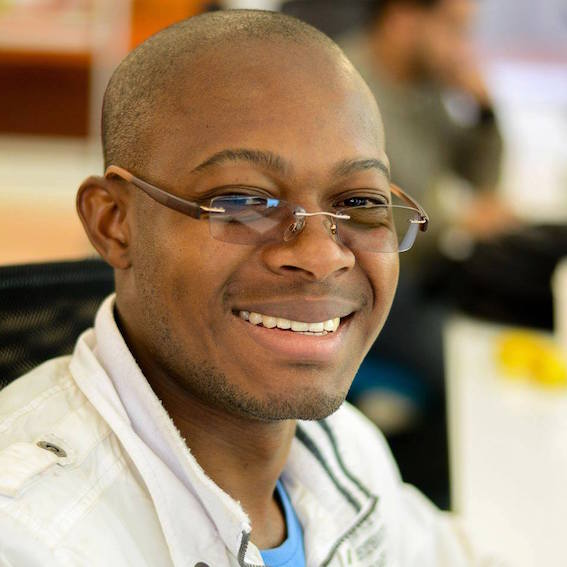
\includegraphics[width=\textwidth,height=.5\textheight]{logo}}
	%\institute{}
	%\date{}
	%\subject{}
	%\setbeamercovered{transparent}
	%\setbeamertemplate{navigation symbols}{}
	\begin{frame}[plain]
	\maketitle
\end{frame}

\begin{frame}
\frametitle{Table of contents}
\begin{itemize}
	\item Definitions: model governance, risk management, model risk
	\item Model governance lifecycle
\end{itemize}
\end{frame}


%\begin{frame}
%\frametitle{Elasticsearch for Hadoop}
%\begin{figure}[h]
%	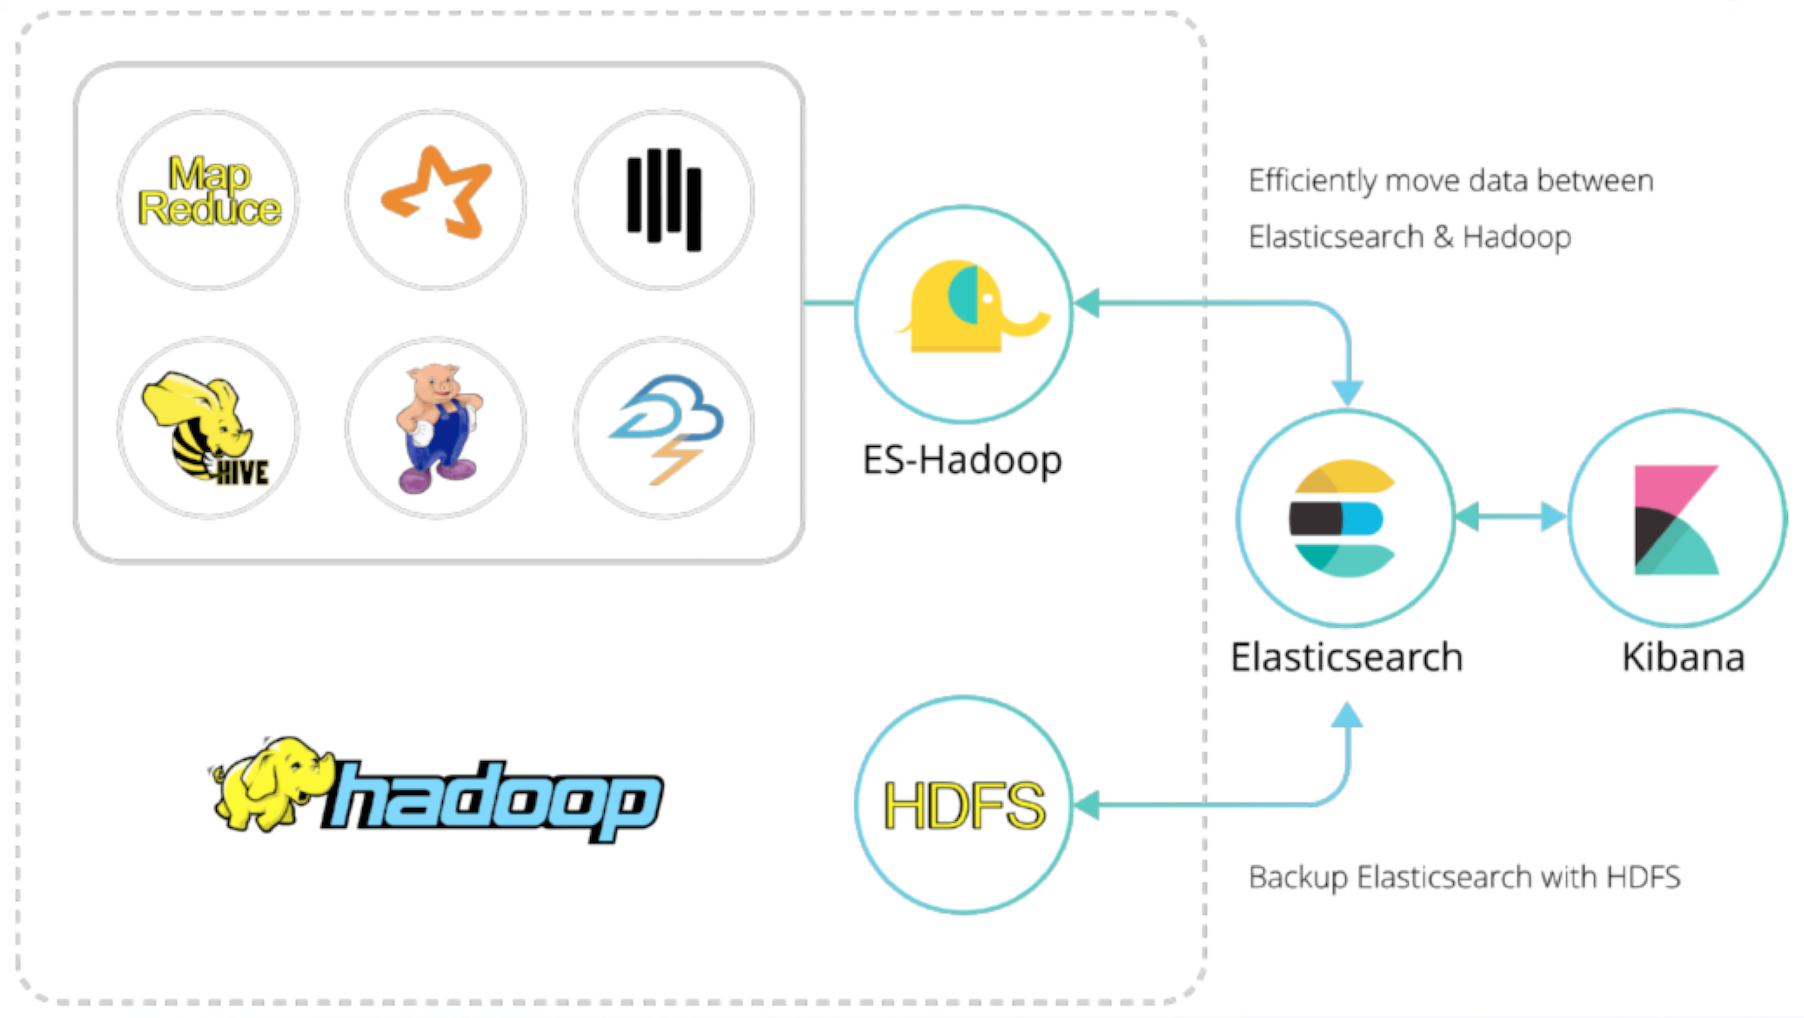
\includegraphics[scale=.3]{images/es_hdp}
%\end{figure}
%\end{frame}
%
%
%\begin{frame}
%\frametitle{Kafka installation}
%\begin{itemize}
%	\item Download the binary: kafka\_2.12-1.0.1.tgz 
%	\item 7z x  kafka\_2.12-1.0.1.tgz \&\& 7z x  kafka\_2.12-1.0.1.tar
%	\item sudo mv kafka\_2.12-1.0.1 /opt/Kafka
%\end{itemize}
%\end{frame}


\begin{frame}
\frametitle{References}
\begin{enumerate}
	\item Building Intelligent Systems: A Guide to Machine Learning Engineering. [Geoff Hulten] (Apress, 2018)
	\item Trends in AI, Data Science, and Big Data. [Ben Lorica] (2017)
	\item Building Evolutionary Architectures. [Rebecca Parsons; Patrick Kua; Neal Ford] (O'Reilly Media, 2017)
	\item 5 things you should be monitoring. [Brian Brazil] (2018)
	\item The Logstash Book. [James Turnbull] (Turnbull Press, 2013)
	\item Beyond the Twelve-Factor App. [Kevin Hoffman] (O'Reilly Media, 2016)
	\item Logs and real-time stream processing. [Jay Kreps] (2016)
	\item I Heart Logs: Apache Kafka and Real-time Data Integration. [Jay Kreps] (2015)
	\item The log: The lifeblood of your data pipeline. [Kiyoto Tamura] (2015)
	\item Understanding the ELK stack. [Brian Anderson; Rafał Kuć] (2016)
\end{enumerate}
\end{frame}

\end{document}